\documentclass[tikz,border=8pt]{standalone}
\usepackage{tikz}
\usetikzlibrary{arrows.meta,calc,patterns}

\definecolor{ink}{HTML}{363636}

\begin{document}
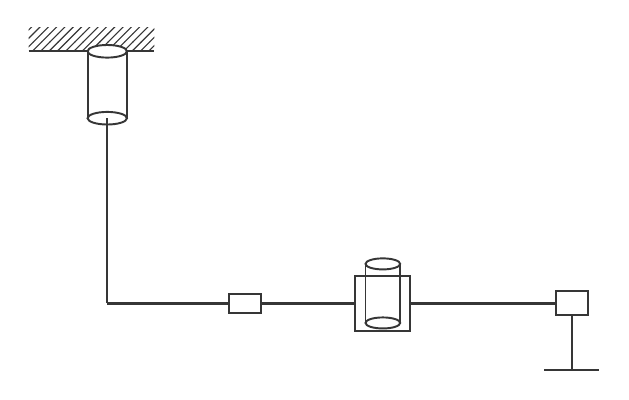
\begin{tikzpicture}[
    line cap=butt, line join=miter,
    link/.style={ink, line width=0.9pt},
    joint/.style={ink, fill=white, line width=0.7pt},
]

% Ceiling (hatched)
\fill[pattern=north east lines, pattern color=ink]
    (-1.0,5.4) rectangle (0.6,5.7);
\draw[ink, line width=0.6pt] (-1.0,5.4) -- (0.6,5.4);

% Base cylinder (joint 1)
\draw[joint] (-0.25,4.55) rectangle (0.25,5.4);
\draw[joint] (0,5.4) ellipse (0.25 and 0.08);
\draw[joint] (0,4.55) ellipse (0.25 and 0.08);

% Vertical link L1
\draw[link] (0,4.55) -- (0,2.2);

% Horizontal link L2
\draw[link] (0,2.2) -- (3.5,2.2);

% Small coupling box on L2
\draw[joint] (1.55,2.08) rectangle (1.95,2.32);

% Joint 3: outer block + revolute cylinder
\draw[joint] (3.15,1.85) rectangle (3.85,2.55);
\draw[joint] (3.5,2.7) ellipse (0.22 and 0.07);
\draw[joint] (3.28,2.7) -- (3.28,1.95);
\draw[joint] (3.72,2.7) -- (3.72,1.95);
\draw[joint] (3.5,1.95) ellipse (0.22 and 0.07);

% Link L3
\draw[link] (3.85,2.2) -- (5.9,2.2);

% End effector / prismatic d4
\draw[joint] (5.7,2.05) rectangle (6.1,2.35);
\draw[link] (5.9,2.05) -- (5.9,1.35);
\draw[link] (5.55,1.35) -- (6.25,1.35);

\end{tikzpicture}
\end{document}
